\documentclass[12pt,a4paper]{exam}
\usepackage[utf8]{inputenc}
\usepackage[french]{babel}
\usepackage[T1]{fontenc}
\usepackage{amsmath}
\usepackage{amsfonts}
\usepackage{amssymb}
\usepackage{graphicx}
\usepackage[left=2cm,right=2cm,top=2cm,bottom=2cm]{geometry}
\title{Composition de physique -- Décembre 2020}
\date{}

\usepackage[thinspace,thinqspace,amssymb]{SIunits}

\begin{document}

\maketitle

\begin{figure}[b!]
\center
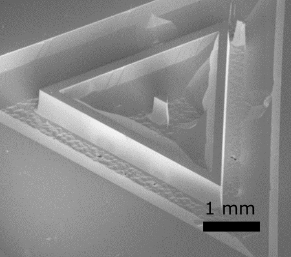
\includegraphics[height=200pt]{figures/micropillar.png}
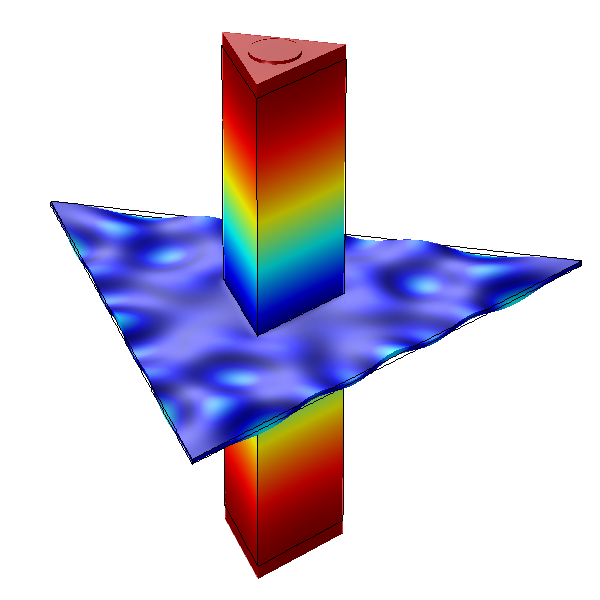
\includegraphics[height=200pt]{figures/micropillar_disp.png}
\caption{Image obtenue par microscopie électronique d'un micro-pilier en quartz.
Seul le déplacement des extrémités du pilier triangulaire au centre est étudié ici.
Le déplacement associé au mode de compression étudié ici peut-être simulé.
La figure de droite montre les résultats d'une telle simulation : les déplacements importants sont indiqués en rouge.}
\label{fig:micro_pillar}
\end{figure}

\section{Oscillateur harmonique -- oscillateur amorti}

Dans le référentiel du laboratoire $\cal{R}$, on considère un système formé d'une masse ponctuelle $m$ accrochée à une extrémité d'un ressort de constante de raideur $k$ et longueur à vide $l_0$.
La masse est astreinte à se déplacer sans frottement sur l'axe $x$ horizontal.
On repère la position de la masse par la coordonnée $x$, avec $x=0$ au repos.

\begin{questions}
\question Faire un schéma.
\question En considérant le référentiel $\cal{R}$ galiléen, faire un bilan des forces.
\question Établir l'équation du mouvement et exprimer la pulsation caractéristique $\Omega_m$ en fonction de $m$ et $k$.
\question Pour tenir compte des phénomènes dissipatifs, on suppose qu'une force de frottement fluide $\overrightarrow{f}=-\alpha\overrightarrow{v}$ s'exerce sur $m$.
Établir la nouvelle équation du mouvement
\question La mettre sous la forme
\begin{equation}
\ddot{x} + \Gamma_m \dot{x} + \Omega_m^2 x = 0,
\label{eq:damped_oscillator}
\end{equation}
et exprimer $\Gamma_m$ en fonction de $\alpha$ et $m$.
\question On suppose que le facteur de qualité $Q=\Omega_m/\Gamma_m$ de l'oscillateur vérifie $Q>\frac{1}{2}$.
Résoudre l'équation obtenue en supposant qu'à l'instant initial la masse se trouve en $x_0$ et qu'on la lâche sans vitesse initiale.
\question Tracer l'évolution temporelle de $x(t)$ en faisant apparaitre les deux temps caractéristiques $T=2\pi/\Omega_m$ et $\tau=2\pi/\Gamma_m$.
%\question Sachant que ce système se comporte comme un filtre passe-bas résonant, tracer qualitativement l'allure de la réponse en déplacement du système à une excitation forcée en faisant apparaitre les pulsations caractéristiques.
\question À quelles conditions sur $\Omega_m$ et $\Gamma_m$ peut on supposer $\cal{R}$ galiléen.
\end{questions}

\section{Le micro-pilier : influence de la masse}

\begin{figure}
\center
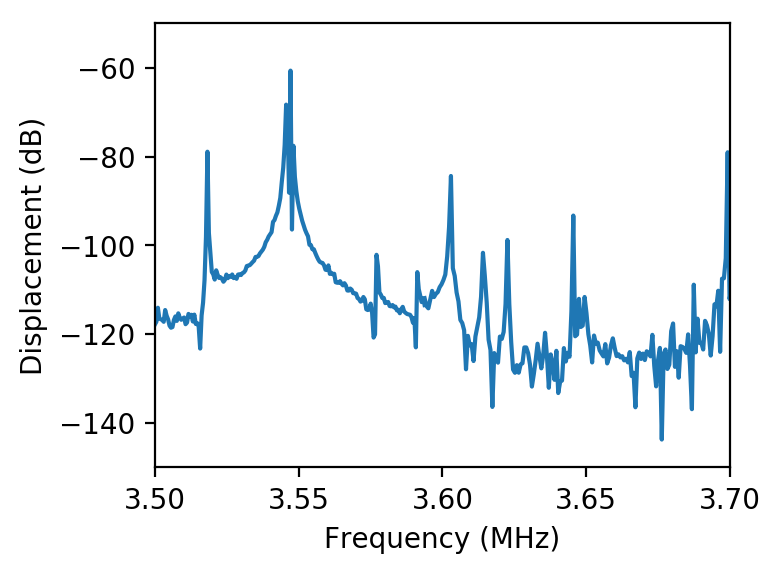
\includegraphics[height=300pt]{figures/broadband_driven_response.png}
\caption{Mesure du déplacement des extrémités du pilier en fonction du temps en régime libre, obtenue après arrêt soudain d'une excitation résonante.}
\label{fig:ringdown}
\end{figure}

On s'intéresse à un micro-pilier en quartz suspendu en son centre par une fine membrane (Fig.~\ref{fig:micro_pillar}).
Les extrémités du pilier se déplacent faiblement symétriquement de part et d'autre de la membrane en raison de l'élasticité du matériau.

\begin{questions}
\question En assimilant le pilier à un cylindre de hauteur $h=\unit{1}{mm}$ et de section circulaire de rayon $r=\unit{90}{\micro\meter}$, donner l'expression de la masse du pilier $m_p$ en fonction de la masse volumique du quartz $\rho_q$.

Faire l'application numérique avec $\rho_q=\unit{2{,}6}{\kilo\gram\per\meter^3}$.
\question Déduire de la Fig.~\ref{fig:ringdown} la période propre et donner la valeur numérique de $\Omega_m$ dans le cas du micro-pilier. 
\question Les déplacements des extrémités du pilier sont bien décrits par l'équation~\eqref{eq:damped_oscillator}, en remplaçant la masse $m$ par $m_p/2$ en raison de la forme du mode de vibration du pilier.
En déduire la constante de raideur $k_p$.
\question Qualitativement, quelle est l'influence d'une augmentation de la masse du système sur la pulsation propre du système ?
Exprimer la variation $\delta\Omega$ due à une augmentation $2\delta m$ de la masse du pilier.
\question On mesure les déplacements du pilier par interférométrie optique ce qui nécessite de déposer un miroir sur l'une des extrémités du pilier.
Pour simplifier, on suppose qu'on ajoute une dépôt diélectrique réfléchissant de masse $\delta m = \unit{50}{\nano\gram}$ sur chacune des extrémités du pilier.
Calculer numériquement le déplacement $\delta\Omega$.
\question Sachant qu'on peut facilement mesurer un déplacement de la pulsation propre de l'oscillateur si $\delta\omega > \Gamma_m$, donner l'expression de la plus petite masse $\delta_m$ qui donne une déplacement en fréquence mesurable.
\question Faire l'application numérique pour le micro-pilier et justifier que ce type de système puisse être utilisé pour réaliser une balance pour la mesure de masses très faibles.
\end{questions}

\section{Le micro-pilier : influence de la pression}

\begin{figure}
\center
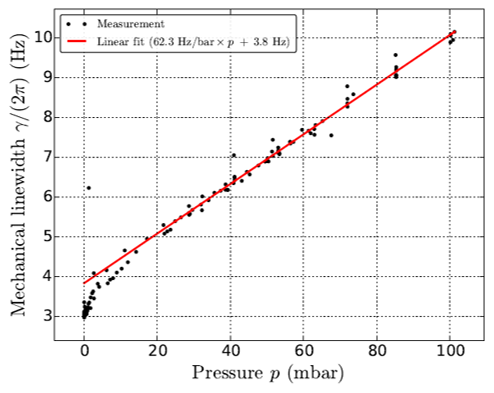
\includegraphics[height=300pt]{figures/gaz_damping.png}
\caption{Évolution de la dissipation mécanique \emph{totale} $\Gamma_m$ en fonction de la pression du gaz environnant.
Les mesures sont réalisées à \unit{300}{\kelvin}.}
\label{fig:gaz_damping}
\end{figure}

Dans le cas du micro-pilier, on suppose que le taux d'amortissement $\Gamma_m$ s'exprime comme la somme de deux termes associés à des processus dissipatifs distincts :
\begin{itemize}
\item dissipation intrinsèque $\Gamma_0$ associées aux pertes dues aux déformations du quartz : elles ne dépendent que du matériau et de la forme du mode ;
\item dissipation acoustique $\Gamma_a(P)$ : les extrémités du pilier mettent en mouvement les particules de fluide du gaz environnant et se comportent comme un minuscule haut-parleur. 
\end{itemize}
Le premier est constant mais le deuxième dépend de la pression du gaz dans lequel est placé l'oscillateur.
On suppose $\Gamma_a(P)$ de la forme
\begin{equation}
\Gamma_a(P) = \beta \frac{\rho_g(P)}{\rho_q},
\end{equation}
où $\beta$ est une constante, $\rho_g(P)$ la masse volumique du gaz et $\rho_q$ la masse volumique du quartz donnée dans la partie précédente.

\begin{questions}
\question Sous quelle forme l'énergie est-elle perdue dans le cas de la dissipation acoustique ?
\question En supposant l'air composé uniquement de diazote de masse molaire $M=\unit{28}{\gram\per\mole}$ et assimilé à un gaz parfait, exprimer sa masse volumique $\rho_a(P)$ en fonction de $P$.
\question D'après les résultats de l'ajustement linéaire de la Fig.~\ref{fig:gaz_damping}, déduire les valeurs numériques de $\Gamma_0$ et $\beta$.
\question En déduire la pression $P_l$ pour laquelle $\Gamma_a(P_l)=\Gamma_0$.
Faire l'application numérique
\question Justifier que ce type de système puisse être utilisé comme capteur de pression.
En exploitant le résultat de la question précédente, quel est l'intérêt d'utiliser un oscillateur avec un grand facteur de qualité ?
\end{questions}

\end{document}